\chapter{Deep integrations on polarization with PAPER-128}
\label{chapter:eor_window_psa128}

In Chapter~\ref{chapter:eor_window_paper32img}, I presented polarized power spectra from a short integration -- a few hours of one night -- over a wide range of $k_{\perp}$-modes probed by the PAPER-32 polarized imaging array \citep{Kohn.16}. Chapter~\ref{chapter:eor_window_HERA} presented the first power spectral results from HERA. The HERA-19 commissioning array was small and dense, meaning that only a few $k_{\perp}$-modes were accessible. For that study, we averaged over 10 hours per night, for 8 consecutive nights \citep{Kohn.18}. This Chapter presents results from the PAPER-128 array. In this Chapter I present roughly one quarter of the total number of observations recorded by this interferometer (Section~\ref{sec:psa128_obs}). I show results of a deep integration on a very narrow range of $k_{\perp}$-modes (corresponding to $\sim$30\,m spacings of the redundant grid; Section~\ref{sec:psa128_results}) and discuss the implications for deep, fully-polarized integrations with large interferometers (Section~\ref{sec:psa128_conc}).

\section{Observations \& Reduction}
\label{sec:psa128_obs}
 
PAPER-128 was the largest build-out of the PAPER experiment. As described in Chapter~\ref{chapter:instruments},  PAPER-128 consisted of 128 antennas, 112 of which were arranged in a redundant grid. An annotated photograph of the array is shown in Figure~\ref{fig:psa128photo}. In this section, I review the PAPER-128 campaign (Section~\ref{subsec:psa128_obs_overview}) and the subsequent reduction of roughly one quarter of the total number of observations (Section~\ref{subsec:psa128_s1e2_reduction}).

\begin{figure}
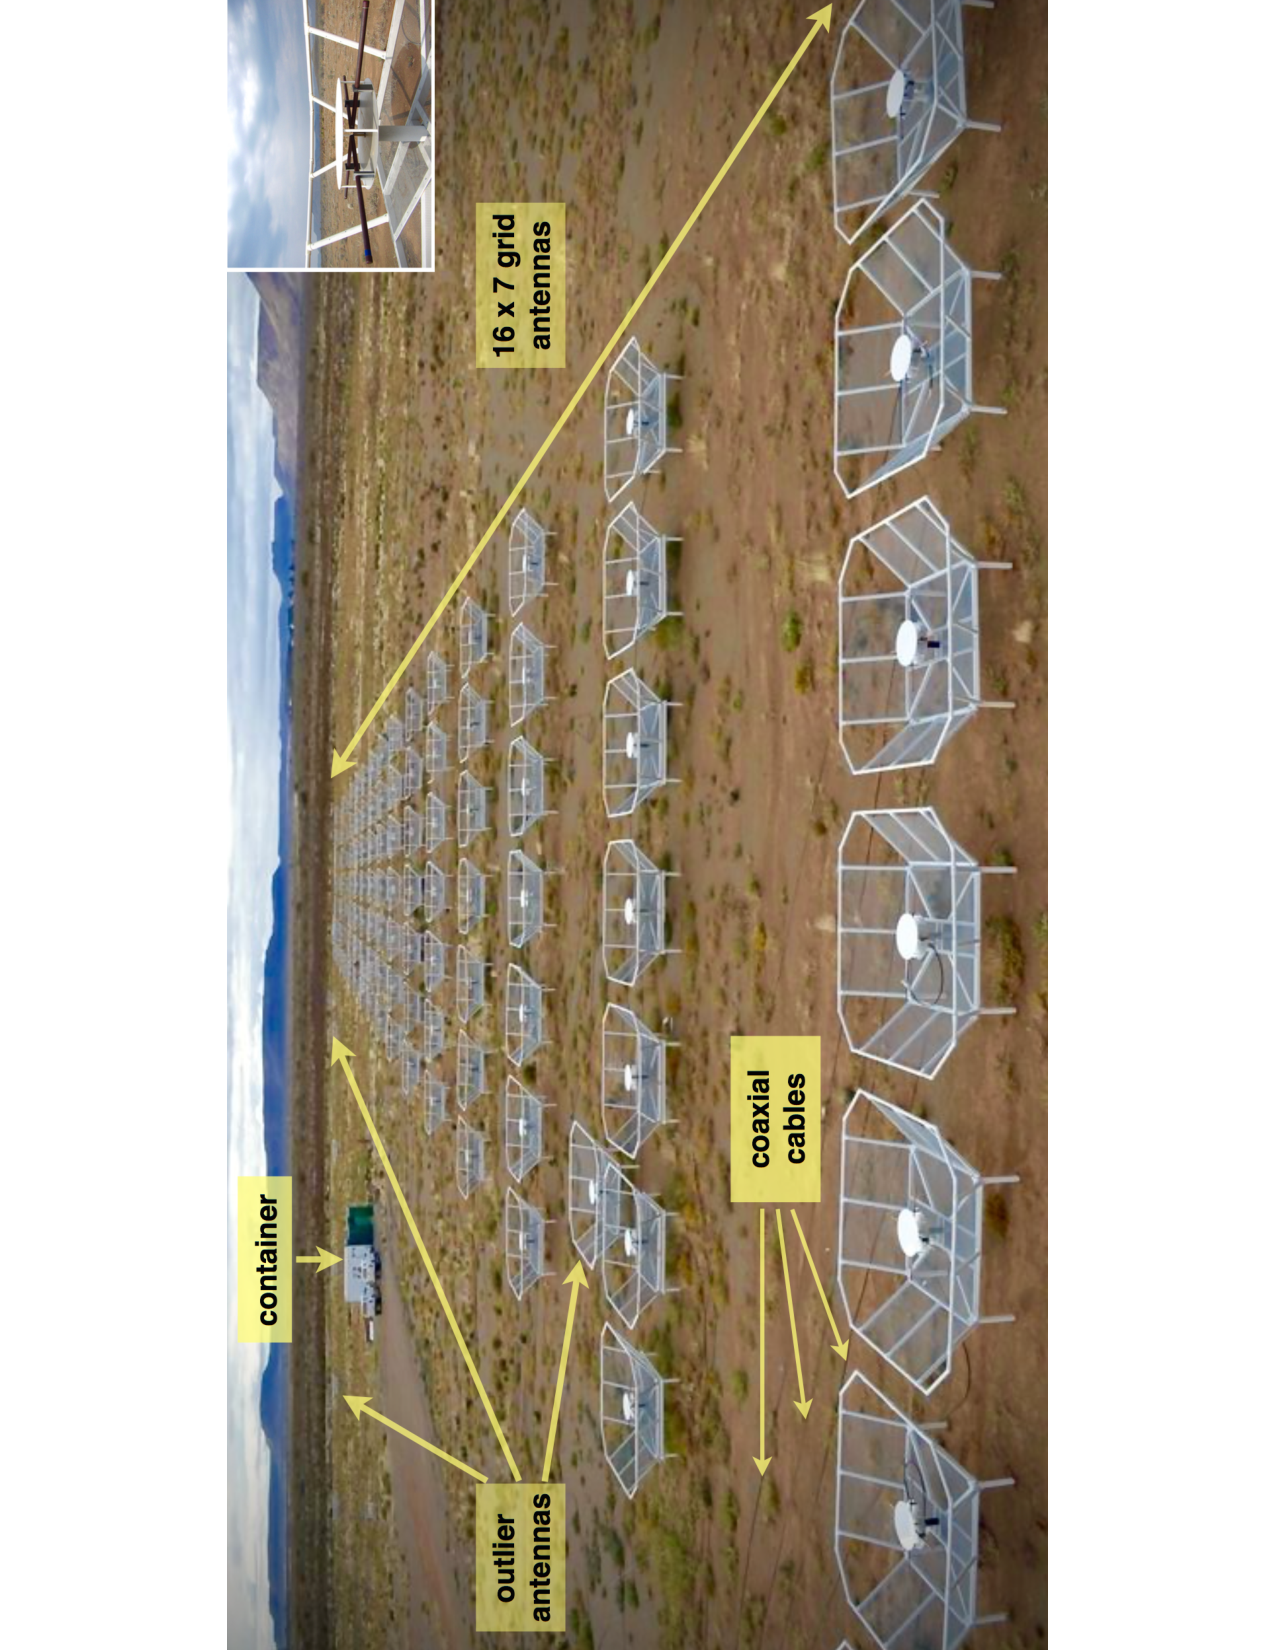
\includegraphics[width=0.8\textwidth, angle=270]{chapters/psa128_pol/figures/array_photo_diagram.pdf}
\caption[An annotated photograph of the PAPER-128 array.]{An annotated photograph of the PAPER-128 array, looking to the East. Highlighted are the 112 antenna redundant grid, with 15\,m East-West spacings between each row; outlier antennas from the main grid used to increase \textit{uv}-coverage; coaxial cables running to the receiverators and correlator (see Chapter~\ref{chapter:instruments}). An inset panel shows a PAPER sleeved dipole. Photo credit: J. E. Aguirre. Figure credit: C. D. Nunhokee; \citep{Nunhokee_thesis}.}
\label{fig:psa128photo}
\end{figure}

\subsection{Overview of PAPER-128 observations}
\label{subsec:psa128_obs_overview}
Observations were recorded for two years, with first light on November 20th 2013 and final readings on January 27th 2015. However, these observations were not always contiguous. Human errors, experimentation and malfunctioning electronics required the correlator and connected electronics to be turned off and restarted, altering the characteristic phasing and gain scale of the array. Each of these restarts constituted the beginning of a new ``Epoch" of the array which required different quality assurance steps and initial calibration stages. Table~\ref{tab:seasons_psa128} summarizes the length and nature of these Epochs. 

\begin{deluxetable}{lllll}
\centering
\label{tab:seasons_psa128}
\tablewidth{0pt}
\tablecaption{PAPER-128 Observing Seasons \& Epochs}
\tabletypesize{\footnotesize}
\tablehead{
\colhead{Season} & \colhead{Epoch} & \colhead{Julian Dates} & \colhead{Calendar Dates} & \colhead{Notes} \\
}
\startdata
1 & 1 & 2456617 - 2456673 & Nov 20, 2013 - Jan 15, 2014 & 1/8 F-Engine failure \\
   & 2 & 2456678 - 2456724 & Jan 20, 2014 - Mar 7, 2014 &  Good \\
2 & 1 & 2456625 - 2456732 & Mar 8, 2014 - Mar 7, 2014 & Too few data \\
   & 2 & 2456843 - 2456873 & Jul 4, 2014 - Aug 3, 2014 & Uninteresting LST range \\
   & 3 & 2456881 - 2456928 & Aug 11, 2014 - Sep 27, 2014 &  Many malfunctioning antennas \\
   & 4 & 2456942 - 2457008 & Oct 11, 2014 - Dec 11, 2014 &  Good \\
   & 5 & 2457030 - 2457050 & Jan 7, 2015 - Jan 27, 2015 &  Many malfunctioning antennas\\
\enddata
\end{deluxetable}

Figure~\ref{fig:psa128_epochs} illustrates the challenge imposed by the correlator restarts. Epoch changes were characterized by large shifts in the overall phase of visibilities, of course leading to changed magnitudes of the real and imaginary parts of the visibilities recorded. The quality assurance metrics described in Chapter~\ref{chapter:data_prep_and_proc} were sensitive to these changes. Of course, absolute calibration -- that is phasing to the correct point on the sky and scaling the visibilities from arbitrary to physical flux density units -- had to be run separately on individual Epochs.

\begin{figure}
\centering
\includegraphics[width=0.7\textwidth]{chapters/psa128_pol/figures/S2_chan100_hist.pdf}
\includegraphics[width=0.5\textwidth]{chapters/psa128_pol/figures/S2_chan100_phasegrid.pdf}
\caption[The challenge of Epoch changes.]{The challenge of Epoch changes. Shown are all of the Season 2 time samples of the visibilities recorded by the 30\,m baseline between antennas 1 and 4, LSTs 0--5, for only the 150\,MHz frequency bin. The above panel shows a histogram of the real part of the visibilities as a function of LST -- there is a dramatic change in magnitude with respect to LST. Likewise, the lower panel shows the phase of each visibility sample (color axis) as a function of LST (vertical axis) and day of observation (x axis). There are obvious large shifts in phase, which require separate calibration stages.}
\label{fig:psa128_epochs}
\end{figure}

As shown in Table~\ref{tab:seasons_psa128}, Season 2 had a larger number of observed nights than Season 1. However, the analysis of Season 2 was especially challenging due to large numbers of malfunctioning antennas. This may have been due to the antennas ageing past a critical point. Nothing in the array was replaced during build-outs except for the correlator; 32 of the antennas had been out in the desert for 4--5 years (PAPER-32) and another 32 for 3--4 years (PAPER-64). Most of the time, these were the antennas that were identified as malfunctioning.

Season 2 Epoch 4 was relatively well-behaved, and may be analyzed in the future. For this work, we concentrated our analysis on Season 1. Season 1 Epoch 2 was ten days shorter than Season 1 Epoch 1, but Epoch 1 had two major challenges associated with it: a data loss event, and an F-engine failure. Due to human error, Epoch 1 data was deleted and had to be restored and recompressed (see Chapter~\ref{chapter:data_prep_and_proc}). This was almost entirely successful, at the loss of one week's worth of observations. The F-engine failure was more critical. We discovered during out analysis that exactly one eighth of the antennas in the array produced noise-like visibilities with the rest of the array, but normal correlations between one another. These antennas had ``seceded" from the array. They shared the characteristic of all being attached to the same F-engine (of which there were eight; see Figure~\ref{fig:instruments_PAPER_Signal_Chain}). This suggested that there was a clock-offset on that F-engine, resulting in no correlation between the signal from those antennas and those running through the other in-sync F-engines.

This left Season 1 Epoch 2 as the most well-characterized and well-behaved Epoch of PAPER-128 observations, and we focused on this Epoch alone from now on. Cross-polarization metrics identified seven incorrectly-rotated antennas, which were corrected during initial processing. Eight antennas were identified as malfunctioning by mean visibility amplitude metrics, including one of those that was incorrectly-rotated. The state of the array for Season 1 Epoch 2 is summarized in Figure~\ref{fig:s1e2_array}.

\begin{figure}
\centering
\includegraphics[width=0.6\textwidth]{chapters/psa128_pol/figures/s1e2_array.png}
\caption[Good, bad and rotated antennas in Season 1 Epoch 2.]{Good, bad (red crosses) and rotated (blue circles) antennas in Season 1 Epoch 2, as identified by the cross-polarization and visibility amplitude metrics defined in Chapter~\ref{chapter:data_prep_and_proc}.}
\label{fig:s1e2_array}
\end{figure}

\subsection{Reduction of Season 1 Epoch 2 data}
\label{subsec:psa128_s1e2_reduction}

After correcting for cross-polarized and malfunctioning antennas, we were able to begin processing the data using the redundant calibration techniques described in Chapter~\ref{chapter:polcal}. We used the phase-flattening algorithm described in Section~\ref{sec:polcal_data} to solve for phase slopes for each antenna. This was performed for the North-South and East-West feed arms separately using the linear instrumental polarizations (`nn' and `ee'), as this method is sensitive to signal-to-noise. We performed a single calculation of these overall delays at the start of the Epoch, and applied those to the rest of the days observed. These overall delays are largely due to electrical delays along the cables leading to the receiverators and the correlator, so we did not expect them to vary a by large amount.

\subsubsection{Redundant calibration}

After phase-wraps were flattened, the {\sc omnical} algorithm could be invoked safely. For this study, we implemented the \textit{4pol+minV} calibration method. For a full exploration of {\sc omnical}ibration methods, see Chapter~\ref{chapter:polcal}. Briefly, the \textit{4pol+minV} calibration scheme redundantly solves for diagonal gains for the North-South and East-West feed arms at the same time, \textit{and} imposes that the `ne' and `en' visibilities are equal. That is, it produces a redundant calibration which minimizes pseudo-Stokes V. Figures~\ref{fig:psa128_pre_post_abs} and \ref{fig:psa128_pre_post_phs} show the successful results of the \textit{4pol+minV} {\sc omnical}ibration, where visibilities from 30\,m East-West baselines showed a high degree of redundancy in all pseudo-Stokes polarizations, and pseudo-Stokes V is almost complete noise-like.

\begin{figure}
\centering
\includegraphics[width=0.8\textwidth]{chapters/psa128_pol/figures/nocal_IQUV_6680_0-5.pdf}
\includegraphics[width=0.8\textwidth]{chapters/psa128_pol/figures/omnical_IQUV_6680_0-5.pdf}
\caption[Amplitudes of three redundant visibilities before and after {\sc omnical}ibration using the \textit{4pol+minV} scheme.]{Amplitudes of three redundant visibilities before (above) and after (below) {\sc omnical}ibration using the \textit{4pol+minV} scheme. All four pseudo-Stokes polarizations attained a high degree of redundancy in magnitude after calibration. The color axis is logarithmic and spans 5 orders of magnitude in arbitrary data units.}
\label{fig:psa128_pre_post_abs}
\end{figure}

\begin{figure}
\centering
\includegraphics[width=0.8\textwidth]{chapters/psa128_pol/figures/nocal_IQUV_6680_phase.pdf}
\includegraphics[width=0.8\textwidth]{chapters/psa128_pol/figures/omnical_IQUV_6680_phase.pdf}
\caption[The same visibilities as shown in Figure~\ref{fig:psa128_pre_post_abs}, but showing their phases instead of their amplitudes.]{The same visibilities as shown in Figure~\ref{fig:psa128_pre_post_abs}, but showing their phases instead of their amplitudes. Again, a high degree of redundancy is obtained between baselines for all polarizations. The color axis is linear and spans $\pi$ (red) to $-\pi$ (blue) radians.}
\label{fig:psa128_pre_post_phs}
\end{figure}

After calibration, we down-selected to only the baselines we sought to analyze for our power spectrum studies. This was partly a utilitarian step: reducing the entire data set would represent a large feat of data processing, since Season 1 Epoch 2 was $\sim2.5$ TB in size if all baselines were retained, and several processing stages that would duplicate the data were still required. The baselines kept were the 30\,m East-West type and their closest diagonals -- that is, 30\,m East-West \& $\pm$4\,m North-South baselines ({\color{red} e.g. Kolopanis et al. (2018)}).

\subsubsection{Foreground removal}
% - linCLEAN
To remove foreground signal from the data, we implemented a variation of the 1D-CLEAN \citep{ParsonsBacker.09} used by past PAPER studies \citep[][{\color{red}; Kolopanis et al. 2018}]{Parsons.14, Ali.15, Jacobs.15, Moore.17, Kerrigan.18}. Instead of performing an iterative CLEAN we used a linear least-squares approach which we termed {\tt linCLEAN}.

Using {\tt linCLEAN}, we endeavoured to model the foreground component of the visibilities using the finite number of Fourier modes that exist within the foreground wedge of the EoR window paradigm. The number of these modes was set by the frequency resolution of the instrument, and the baseline length (see Chapter~\ref{chapter:eor_window_theory}).

We constructed a visibility $\vec{m}(\nu)$ as a model, per time integration, of an individual visibility $\vec{d}(\nu)$ (which we represent as a vector along the frequency axis), seeking to minimize the chi-square

\begin{equation}
\chi^2(\nu) = (\vec{d}(\nu) - \textbf{A}(\nu',\tau)\vec{m}(\nu))^T \textbf{W}(\nu',\nu)(\vec{d}(\nu) - \textbf{A}(\nu,\tau)\vec{m}(\nu)).
\label{eq:linclean_chisquare}
\end{equation}

In the above equation, the matrix $\textbf{A}$ had dimensions ``number of frequency channels" by ``number of allowed delay modes". An allowed delay mode $\tau$ was within the interval [0,  $\frac{|\vec{b}|}{c} + t_{SH}$], for baseline vector $\vec{b}$, speed of light $c$ and an allowed ``supra-horizon leakage" term $t_{SH}$ \citep{Pober.13}, which we set to 15ns.

The contents of $\textbf{A}$ were the concatenation of matrices $\textbf{C}$ and  $\textbf{S}$:
\begin{eqnarray}
\textbf{C}_{ij} &=  \cos(2\pi \nu_i \tau_j)\\
\textbf{S}_{ij} &=  \sin(2\pi \nu_i \tau_j)\\
\end{eqnarray}
for frequency channel $i$ and delay bin $j$.
The matrix $\textbf{W}$ was diagonal, and assigned weighting per frequency channel. With an estimated system temperature one could implement an inverse variance weighting per frequency channel, but we pursued a simpler scheme where the entries were zero for RFI-flagged channels, and unity otherwise.

This system was least-squares solvable for the $\tau$ modes, and granted a foreground model

\begin{equation}
\vec{m}(\nu) = (\textbf{A}^T \textbf{W} \textbf{A})^{-1}\textbf{A}^T\textbf{W}\vec{d}(\nu)
\end{equation}
which could subsequently be subtracted from the $\vec{d}(\nu)$, leaving only the noise-like backgrounds.

\subsubsection{Binning in LST}

After running {\tt linCLEAN} on the Epoch, we implemented a round of RFI flagging that clipped any samples that represented $>4\sigma$ fluctuations above the average, where averages were performed along the time and frequency axes.
We could then average-down on the noise by binning visibilities according to the LST they were observed at. The LST bin size used was 41s long, and we split the Epoch into even and odd days, constructing two separate LST-binned data sets. Cross-multiplying these allowed us to construct an unbiased power spectrum estimate \citep[e.g.][{\color{red}; Cheng et al. 2018}]{Parsons.14}.
Unflagged RFI events would dominate any other signal in a given LST bin. To avoid binning RFI with sky signal, before averaging we computed the median of all observations in a given LST bin and flagged any observations with amplitude $>3\sigma$ above the median. This clipping narrowed the distribution of visibilities about the median, altering the thermal noise variance, but leaving the expectation value unchanged, so we expect little loss of signal due to this step.

For this analysis, we created two LST-binned data sets (each split into even and odd days): a set constructed from the foreground subtracted visibilities, and another set with the foregrounds included. We used the latter to calculate an absolute calibration of both data sets.

\subsection{Absolute calibration \& fringe-rate filtering}
% - (unpolarized) PicA (Jacobs13) CASA cal on lstbin_fg
% - Stokes I FRF on all 4pols of fgsub
We formed images of the Pictor A transit in order to derive an absolute calibration for the `n' and `e' feed arms in the fashion described in Chapter~\ref{chapter:polcal}. We converted the {\sc miriad} files of the LST-binned foreground data into {\tt CASA} \citep{casa} Measurement Sets at LST$\approx$5.3 hours (the relevant LST for the transit of Pictor A). 
Our sky model consisted only of Pictor A as a unpolarized point source. Because we had already down-selected to the power spectrum baselines, Pictor A completely dominated the signal. The images of the four pseudo-Stokes parameters we obtained are shown in Figure~\ref{fig:psa128_abscal_images}. In that image, pseudo-Stokes I is on a color scale with double the dynamic range of Q, U and V -- that is, pseudo-Stokes Q, U and V were almost completely noise-like. In pseudo-Stokes I, Pictor A dominated the field. These images were low quality because only the power spectrum baselines were used to produce the image, leading to large grating lobes and an elongated point-spread function; shown in Figure~\ref{fig:psa128_psf}.

\begin{figure}
\hspace{-2cm}\begin{tabular}{ll}
\includegraphics[clip, trim=0.5cm 9cm 5cm 5cm, width=0.6\textwidth]{chapters/psa128_pol/figures/pretty_I_0-022.pdf} &
\includegraphics[clip, trim=0.5cm 9cm 5cm 5cm, width=0.6\textwidth]{chapters/psa128_pol/figures/pretty_Q_0-011.pdf}\\
\includegraphics[clip, trim=0.5cm 9cm 5cm 5cm, width=0.6\textwidth]{chapters/psa128_pol/figures/pretty_U_0-011.pdf} &
\includegraphics[clip, trim=0.5cm 9cm 5cm 5cm, width=0.6\textwidth]{chapters/psa128_pol/figures/pretty_V_0-011.pdf} \\
\end{tabular}
\caption[Images of Pictor A, used to calibrate the absolute scaling to physical units.]{Images of Pictor A, used to calibrate the absolute scaling to physical units. These images are multi-frequency syntheses, but we used per-channel information for the final calibration (see Figure~\ref{fig:psa128_bandpases}). 
Pseudo-Stokes I is on a linear scale of twice the dynamic range of pseudo-Stokes Q, U and V. A beam ellipse is shown in the South-West corner of the images.
The poor quality of the images is a result of using only the baselines that go into the power spectrum estimates. Pictor A dominates the field in pseudo-Stokes I, and is of the morphology expected given the PSF shown in Figure~\ref{fig:psa128_psf}.}
\label{fig:psa128_abscal_images}
\end{figure}

\begin{figure}
\centering
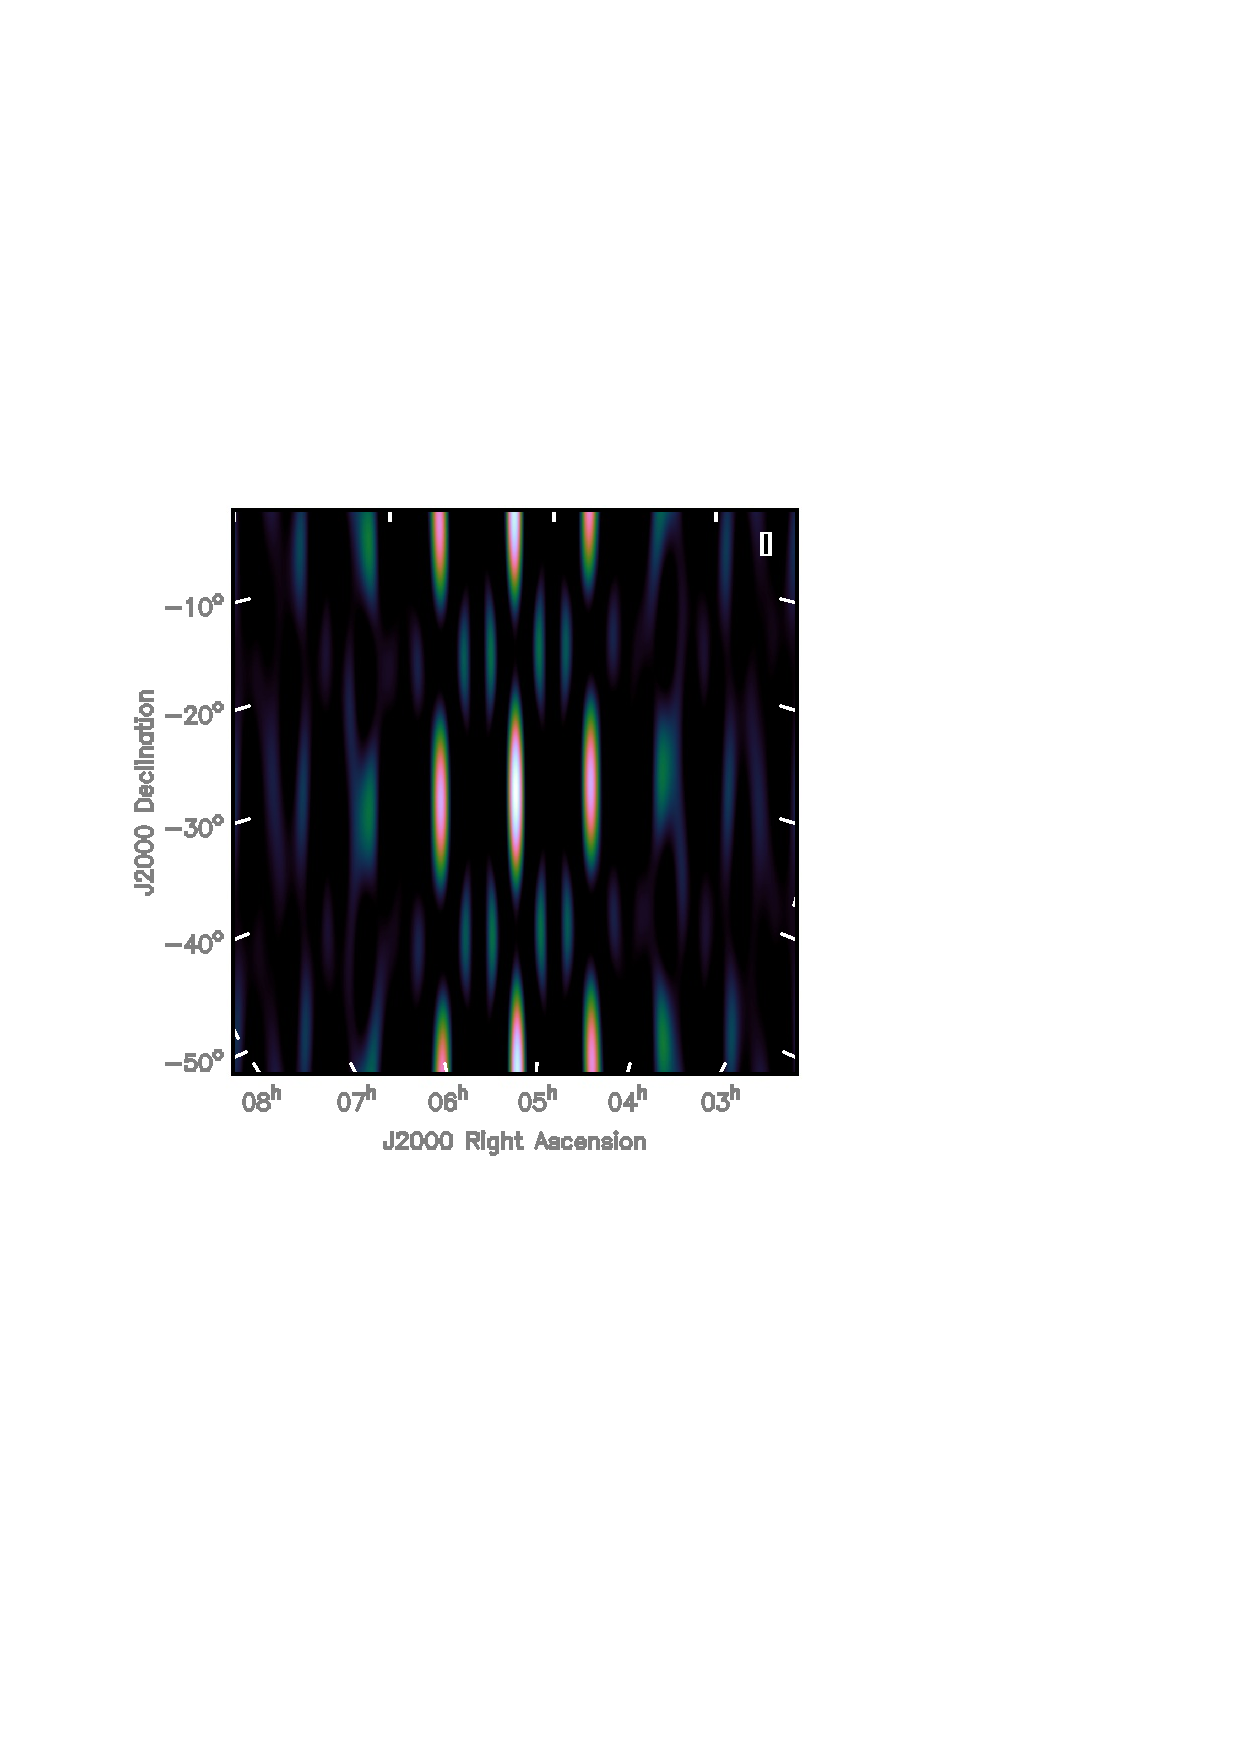
\includegraphics[clip, trim=0.5cm 9cm 5cm 5cm, width=0.6\textwidth]{chapters/psa128_pol/figures/pretty_PSF_0-1.pdf}
\caption[The point-spread function of an array consisting only of the $\sim$30\,m power spectrum baselines.]{The point-spread function of an array consisting only of the $\sim$30\,m power spectrum baselines. The sparseness and asymmetry of the array lead to an elongated PSF with large grating lobes.}
\label{fig:psa128_psf}
\end{figure}

We used the {\tt CASA} {\tt bandpass} routine to derive an overall frequency-dependent scaling that brought the North-South and East-West dipole arms to a physical scale that minimized pseudo-Stokes Q in Pictor A, and converted the data units to a physical level in Janskies. For the Jansky scaling we used the spectrum from \cite{Jacobs.13}. {\tt CASA} provided separate scalings for all antennas used in the analysis. We plot the average scaling for the North-South and East-West dipole arms in Figure~\ref{fig:psa128_bandpases}, shading-in the standard deviation between antennas. We implemented aggressive RFI flags, leading to large gaps in the spectrum. The higher frequency portion of the band had a very low variance its bandpass solutions, as expected given that they were {\sc omnical}ibrated and that the low band was historically poorly-behaved and characterized (e.g. Chapter~\ref{chapter:polcal}).

\begin{figure}
\centering
\includegraphics[width=0.8\textwidth]{chapters/psa128_pol/figures/avg_bandpasses.pdf}
\caption[The average bandpass scaling used for absolute calibration.]{The average bandpass scaling used for absolute calibration, with shading indicating the 1$\sigma$ deviation about the average across antennas.}
\label{fig:psa128_bandpases}
\end{figure}


\section{Results}
\label{sec:psa128_results}

% note -- use high half of the band because reasons e.g. bandpass
% - not-that-great power spectra

\section{Discussion \& Conclusions}
\label{sec:psa128_conc}
% Pitch to "future work", to end the section
% -- levels predicted for detection of Q,U: Nunhokee, Asad
% -- challenges associated with very long integrations: QUALITY ASSURANCE, instrument stability
% -- ionosphere
